\begin{questions}
\question
\textbf{Introduction}

The fundamental matrix F completely describes the epipolar geometry of a pair of images. 8-Point Algorithm is the simplest method for estimating the fundamental matrix. In this assignment, you will implement the 8-Point Algorithm to estimate the fundamental matrix given a pair of images. You would also need to implement the normalization so as to improve the stability (outlined in steps $4.2.2$ and $4.2.4$ below). Finally, we have also provided a package to help you reconstruct and visualize the depths (see point $6$ in $4.3$; this step is optional but will earn you bonus point). Please read this document completely before starting work. A list of reading materials you may need to solve this problem is given in Appendix I.

\question
\textbf{Tasks}

You are given 2 pairs of images (inria1.tif, inria2.tif, frc1.tif, frc2.tif) for this assignment. The steps for this assignment are:
\begin{enumerate}
    \item 
    Using one of the given pairs of images, establish $n (n \geq 8)$ point correspondences.
    
    \item
    Normalize the coordinates of the correspondences.
    
    \item
    Using the normalized coordinates of the correspondences, compute the fundamental matrix.
    
    \item
    Perform denormalization so as to find the fundamental matrix corresponding to the original data.
\end{enumerate}
Details of each step are given in the following sections. Some useful Matlab commands are given in Appendix II.

\begin{parts}
\part
\textbf[Establish Point Correspondences] \\
In this step, you need to establish point correspondences between the two images. Using Matlab, manually or automatically mark and record at least 8 pairs of corresponding points (preferably much more than 8 pairs for robustness!).

\begin{solution}
    After researching online, I used feature matching function provided in Matlab Computer Vision System toolbox based on \textbf{Harris Features} to \textbf{automatically} extract feature-matched points:
    
    \begin{lstlisting}
I1 = imread('frc1.jpg');
I2 = imread('frc2.jpg');

points1 = detectHarrisFeatures(I1, 'MinQuality', 0.001);
points2 = detectHarrisFeatures(I2, 'MinQuality', 0.001);

[features1,valid_points1] = extractFeatures(I1,points1);
[features2,valid_points2] = extractFeatures(I2,points2);

indexPairs = matchFeatures(features1,features2);

matchedPoints1 = valid_points1(indexPairs(:,1),:);
matchedPoints2 = valid_points2(indexPairs(:,2),:);


rand1 = randsample(32, 8);
grp1a = matchedPoints1(rand1);
grp1b = matchedPoints2(rand1);
grp1a = grp1a.Location;
grp1b = grp1b.Location;

rand1 = randsample(32, 8);
grp2a = matchedPoints1(rand1);
grp2b = matchedPoints2(rand1);
grp2a = grp2a.Location;
grp2b = grp2b.Location;

rand1 = randsample(32, 8);
grp3a = matchedPoints1(rand1);
grp3b = matchedPoints2(rand1);
grp3a = grp3a.Location;
grp3b = grp3b.Location;
    \end{lstlisting}
    Running the scripts above, I obtained three sets of points, each of which contains 8 point correspondences. As required by the question, I repeated the process of computing the fundamental matrix to check for the accuracy.
    
    The Figure $9 - 11$ below shows three different sets of matched points. These points are all corresponding \textbf{corners} on both images. They are chosen as the feature points to do the matching since they are less ambiguous compared to plain areas or edges.
    
    \begin{figure}[H]
        \centering
        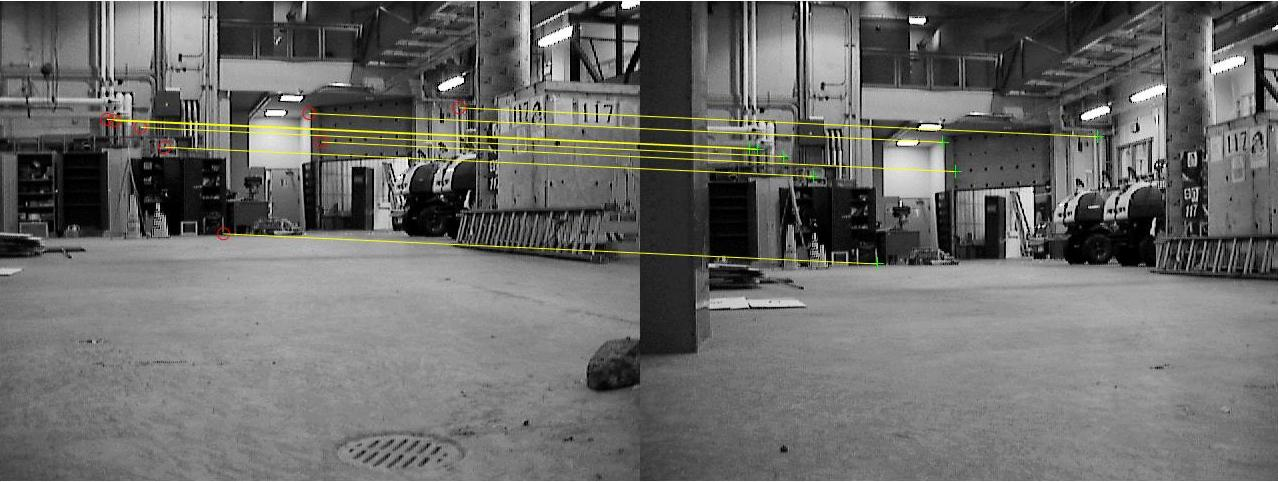
\includegraphics[width=0.75\textwidth]{grp1.jpg}
        \caption{$1 ^{st}$ set of point correspondences}
        \label{fig:mesh1}
    \end{figure}
    
    \begin{figure}[H]
        \centering
        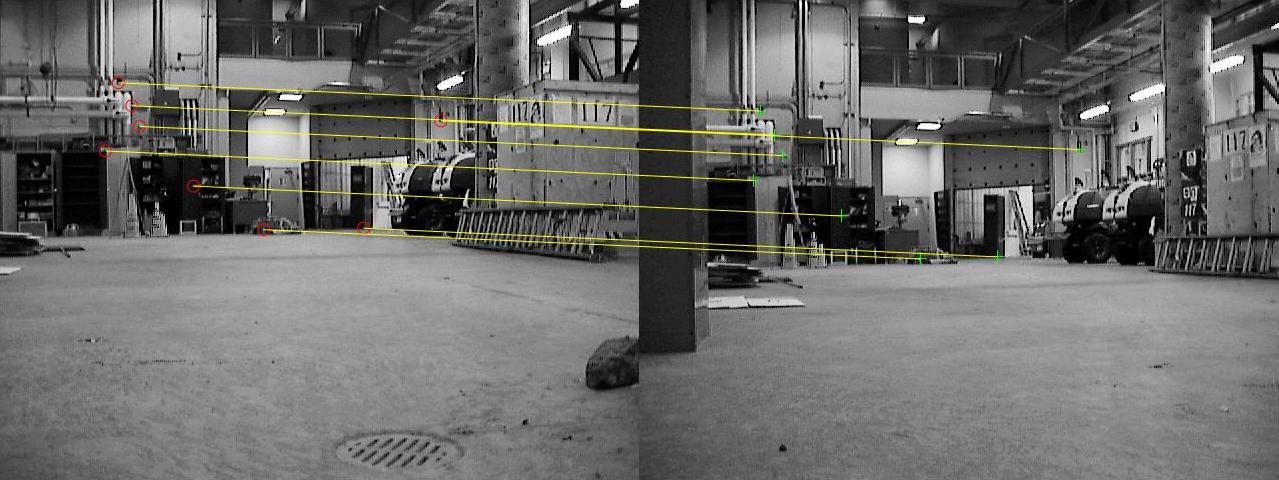
\includegraphics[width=0.75\linewidth]{grp2.jpg}
        \caption{$2 ^{nd}$ set of point correspondences}
    \end{figure}
    
    \begin{figure}[H]
        \centering
        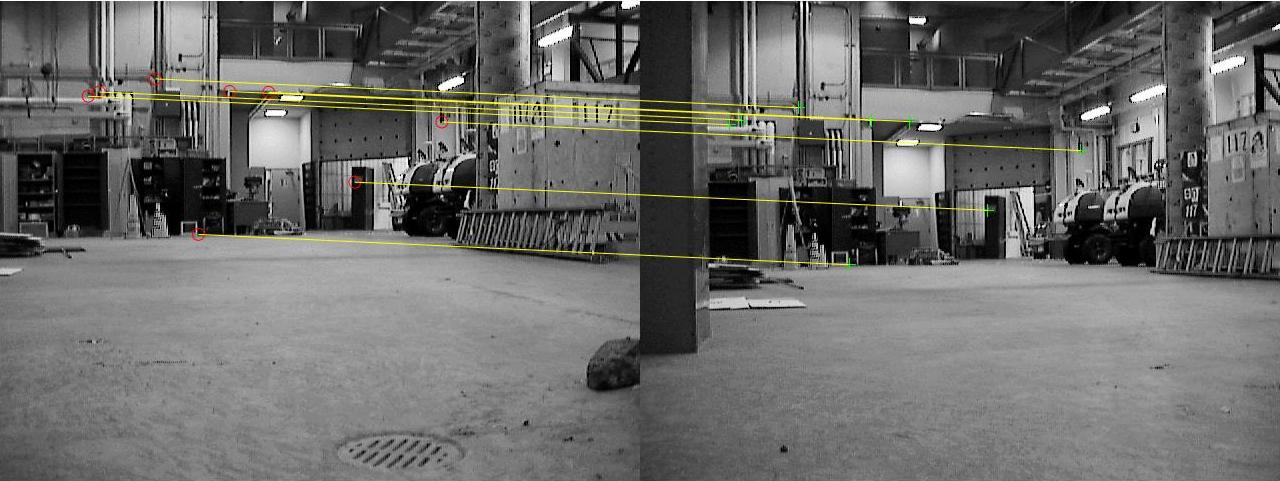
\includegraphics[width=0.75\linewidth]{grp3.jpg}
        \caption{$3 ^{rd}$ set of point correspondences}
    \end{figure}
    
\end{solution}

\part
\textbf[Normalization of the data] \\
In 8-point algorithm, the stability of the results can be greatly improved by a simple normalization (translation and scaling) of the coordinates of the correspondences (originally presented in [Hartley- 1997] and also in [Hartley and Zisserman-2000]). For this normalization, you should find a similarity transformation $T$ , consisting of a translation and scaling, that takes points $x_{i}$ to a new set of points $\hat{x} _ {i}$ ($\hat { x } _ { i } = T x _ { i }$ )such that the centroid of the points $\hat { x } _ { i }$ is the coordinates origin, and their average distance
(Root Mean Squares) from the origin is $2$ pixels . Similarly, find a similarity transformation $T'$ that takes points $x' _ {i}$ to points $xˆ_{i}$ ($\hat {  { x } } _ { i } ^ { \prime } = T ^ { \prime }  { x } _ { i }$).
Note: Homogeneous coordinates are used in this step.
\begin{solution}
    For one image, the centroid of all points is defined by:
    \begin{equation}
        (x_{c}, y_{c}) = (\frac{1}{N} \sum ^ {N} _ {i=1} x _ {i}, \frac{1}{N} \sum ^ {N} _ {i=1} y _ {i})
    \end{equation}
    Every point is translated such that the centroid of the points becomes the coordinate origin. The translation is determined by the centroid's coordinates:
    \begin{equation}
    \begin{split}
        t_{x} = - &x _{c}, \quad t_{y} = - y _{c} \\
        x _ {i} &:= x_{i} + t_{x} \\
        y _ {i} &:= y_{i} + t_{y} \\
    \end{split}
    \end{equation}
    
    After the translation, all the points are scaled such that their Root Mean Square distance from the origin is $\sqrt{2}$, which is equivalent to be scaled by $s$:
    \begin{equation}
        s = \sqrt{\frac{2}{\frac{1}{N} \sum ^ {N} _ {i=1} (x_{i} ^ {2} + y_{i}^{2})} }
    \end{equation}
    Hence, to write the transformation $\hat{x} _ {i} = s (x_{i} + t_{x})$ and $\hat{y} _ {i} = s (y_{i} + t_{y})$ in matrix form:
    \begin{equation}
        T _ {s} = 
        \begin{bmatrix}
        s & 0 & st_{x} \\
        0 & s & st_{y} \\
        0 & 0 & 1
        \end{bmatrix}
    \end{equation}
    The Matlab codes are listed in the next sectioon together with the codes for $F$ estimation.
   
\end{solution}

\part
\textbf[Computation of Fundamental Matrix] \\
The computation of the fundamental matrix is described in detail in your textbook or in Section 10.1 of [Hartley and Zisserman-2000]. In summary the steps are as follows:
\begin{subparts}
    \subpart
    Find the solution for $f$ \\
    From a set of n point correspondences, we obtain a set of linear equations of the form:
    \begin{equation}
        A f = \left[ \begin{array} { c c c c c c c c c} { x^ { \prime } _ { 1 } x _ { 1 } } & { x^ { \prime } _ { 1 } y _ { 1 } } & { x _ { 1 } ^ { \prime } } & { y _ { 1 } ^ { \prime } x _ { 1 } } & { y _ { 1 } ^ { \prime } y _ { 1 } } & { y _ { 1 } ^ { \prime } } & { x _ { 1 } } & { y _ { 1 } } & { 1 } \\ { \vdots } & { \vdots } & { \vdots } & { \vdots } & { \vdots } & {\vdots } & { \vdots }& { \vdots } & { \vdots } \\ { x^ { \prime } _ { n } x _ { n } } & { x^ { \prime } _ { n } y _ { n } } & { x _ { n } ^ { \prime } } & { y _ { n } ^ { \prime } x _ { n } } & { y _ { n } ^ { \prime } y _ { n } } & { y _ { n } ^ { \prime } } & { x _ { n } } & { y _ { n } } & { 1 } \end{array} \right] f = 0
    \end{equation}
    
    $A$ is an $n \times 9$ matrix ($n \geq 8$)and $f$ is the 9-vector made up of the entries of $F$ in row-major order. If $rank(A) \leq 8$, non-trivial solution for the system above exists, and if $rank (A) = 8$ , the solution is unique (up to scale). The solution for $f$ should be the last column of $V$ in the $svd(A) = U \Sigma V^{T}$ .
    
    \subpart
    Enforce singularity constraint\\
    Fundamental Matrix is singular, in fact of rank 2. The matrix $F$ found by the above method will not in general have rank 2 and steps should be taken to enforce this singularity constraint. One easy way to do this is: let $F=U \Sigma V^{T}$ be the SVD of $F$, where $\Sigma$ is a diagonal matrix $diag(r,s,t)$ satisfying $r \geq s \geq t$. Let
    $F^{\prime}=U diag(r,s,0) V^{T}$ . According to the so-called Frobenius norm, $F^{\prime}$ is the closest singular matrix to $F$. Thus replace $F$ by $F^{\prime}$. Note that you should use the normalized data.
    \begin{solution}
        The codes are listed as follows:
        \begin{lstlisting}
% construct A; assume normalized points are stored in n_pts1 and n_pts2
A = [n_pts2(:,1).*n_pts1(:,1) n_pts2(:,1).*n_pts1(:,2) n_pts2(:,1) n_pts2(:,2).*n_pts1(:,1) n_pts2(:,2).*n_pts1(:,2) n_pts2(:,2) n_pts1(:,1) n_pts1(:,2) ones(size(n_pts1(:,1)))];
% from svd(A), get F
[U, S, V] = svd(A);
F = V(:,length(V));
F = reshape(F, [3,3])';
% enforce F singularity
[U_f, S_f, V_f] = svd(F);
S_f(3,3) = 0;
F_prime = U_f * S_f * V_f';
        \end{lstlisting}
    \end{solution}
    
    \subpart
    Denormalization\\
    Till this step, you have obtained the fundamental matrix corresponding to the normalized data $\hat {  { x } } _ { i } \leftrightarrow \hat { { x } } ^ {\prime}_ { i }$. This needs to be denormalized. Set $F = T_{s} ^ {\prime T } F ^ { \prime } T_{s}$ ($T_{s}$ and $T_{s} ^ {\prime}$ is obtained in the normalization step), then $F$ is the fundamental matrix corresponding to the original data $ {  { x } } _ { i } \leftrightarrow  { { x } } ^ {\prime}_ { i }$
    
    \begin{solution}
        The Matlab command simply runs as follows:
        \begin{lstlisting}
F = T_s2' * F_prime * T_s1;
        \end{lstlisting}
        And the result for the fundamental matrix is calculated as:
        \begin{equation}
            F _ {1} = \left[\begin{array} { ccc } { - 5.4958 e - 07 } & { - 4.9610 e - 06 } & { 2.3606 e - 03 } \\ { 3.1570 e - 06 } & { - 1.7717 e - 06 } & { 2.0223 e - 03 } \\ { - 1.6578 e - 03 } & { - 8.4793 e - 04 } & {- 1.4653 e - 01 } \end{array}\right]
        \end{equation}
        During the testing, I found that the epipolar lines do not correspond to the points as shown in the figure below.
            \begin{figure}[H]
                \centering
                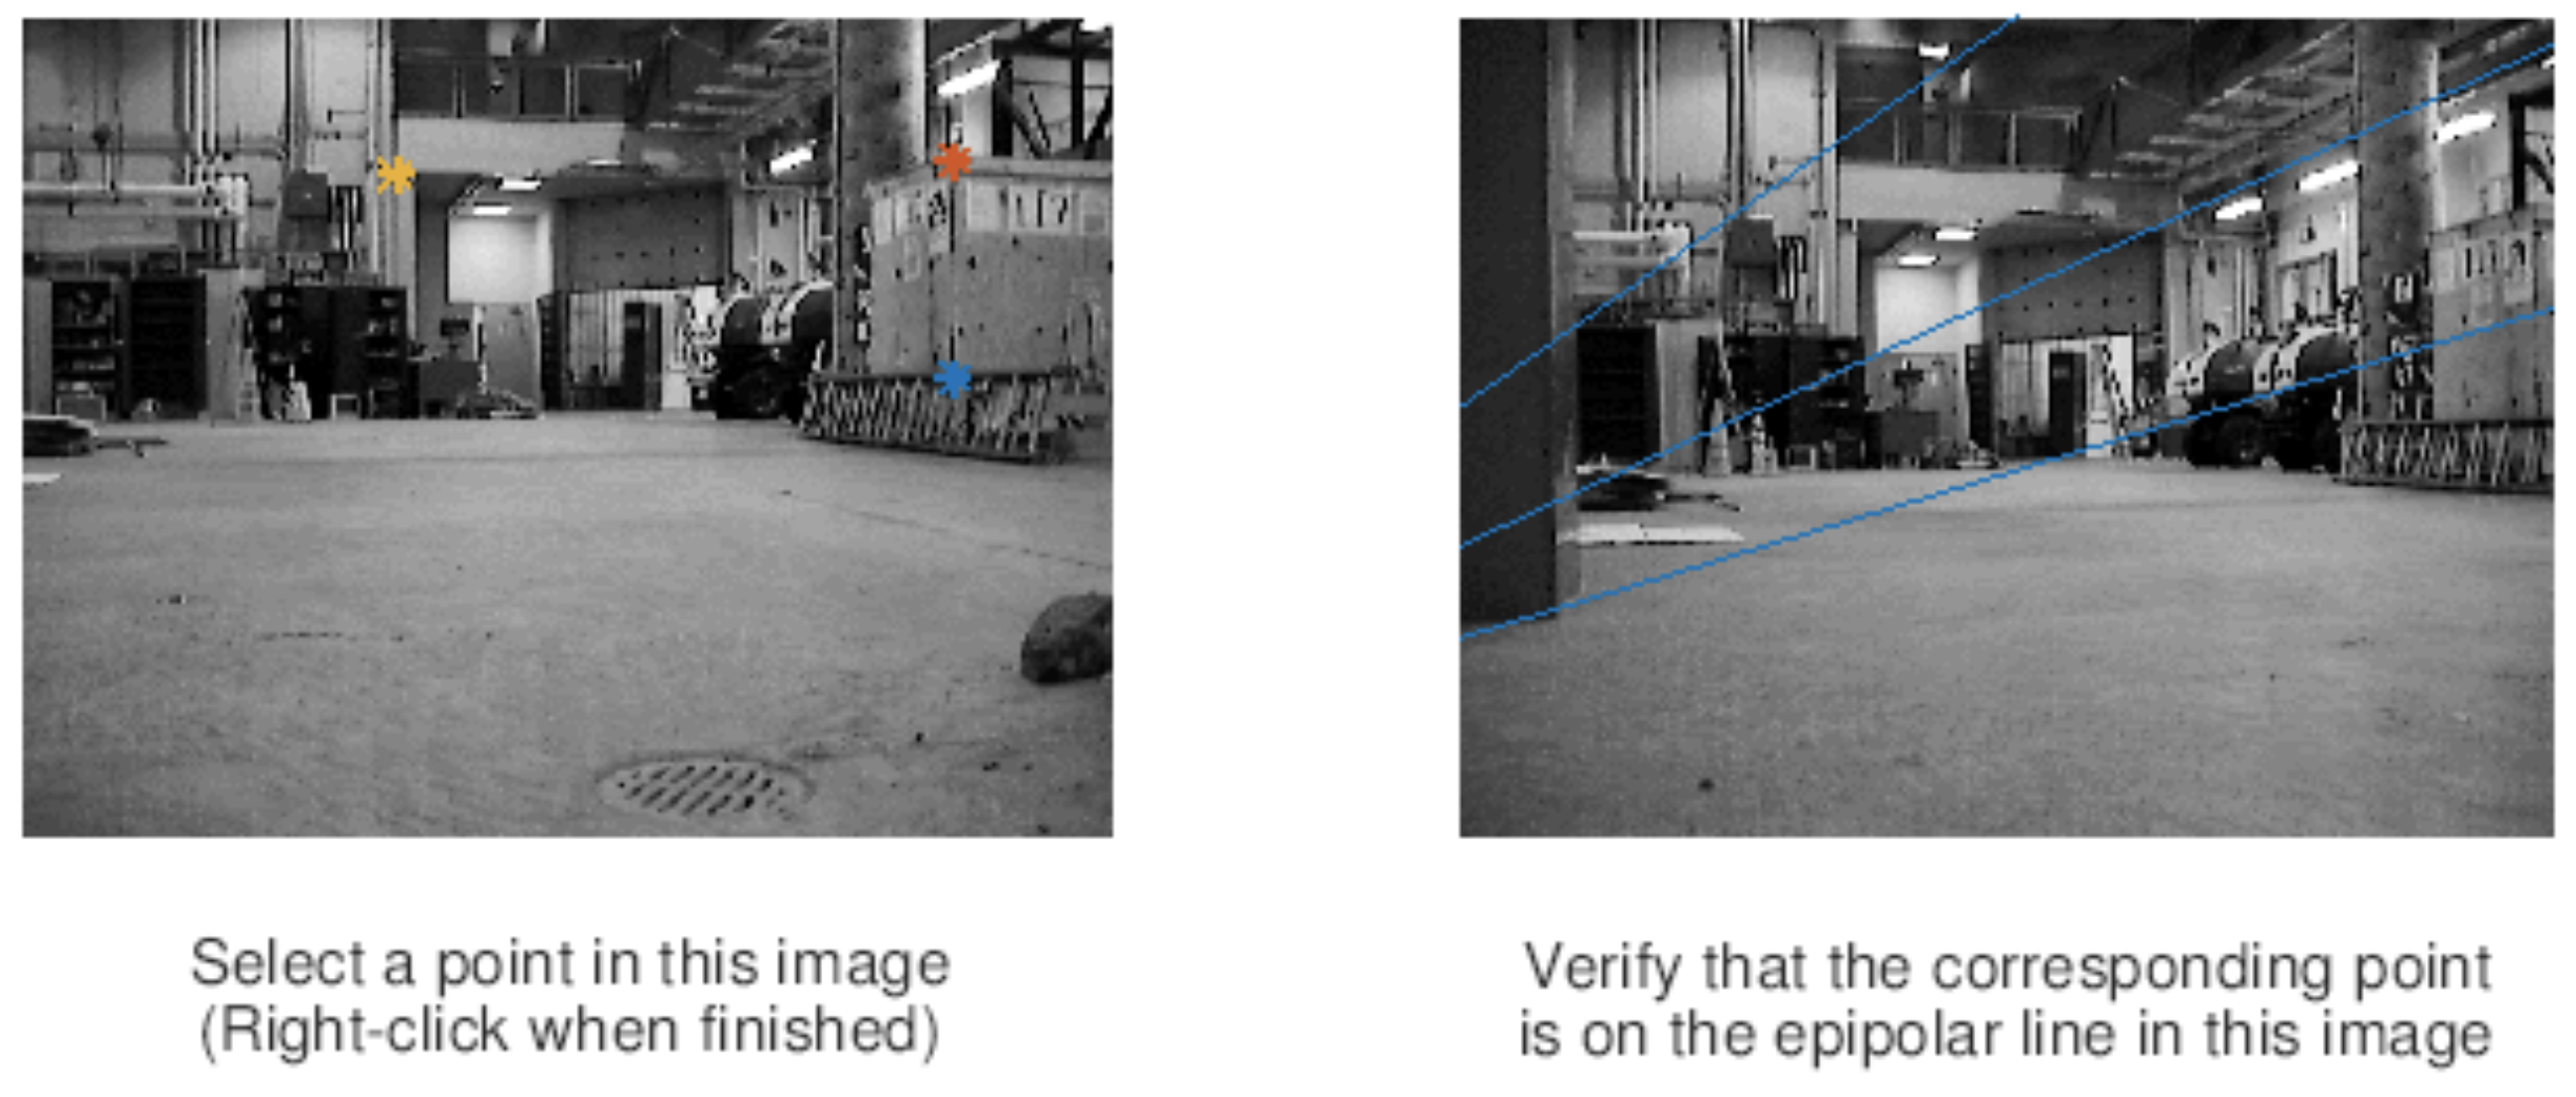
\includegraphics[width=0.85\linewidth]{1st_set_result.png}
                \caption{Epipolar lines found by $l_{r} = Fp_{l}$ ($1^{st}$ set)}
            \end{figure}
        For the second round, I think it will be better if I include more than 8 points. Hence, I concatenated the remaining two sets of data and computed the fundamental matrix again. The calculated fundamental matrix and testing result is shown in the figure below:
        \begin{equation}
            F _ {2} = \left[\begin{array} { ccc } { 4.6784 \mathrm { e } - 10 } & { - 9.2670 \mathrm { e } - 07 } & { 1.3625 \mathrm { e } - 04 } \\ { 7.0476 \mathrm { e } - 07 } & { 1.2601 \mathrm { e } - 07 } & {- 1.7650  \mathrm { e } - 03 } \\ { - 1.2534 \mathrm { e } - 04 } & { 1.7892 \mathrm { e } - 03} & { 4.5285 \mathrm { e } - 02 } \end{array}\right]
        \end{equation}
            \begin{figure}[H]
                \centering
                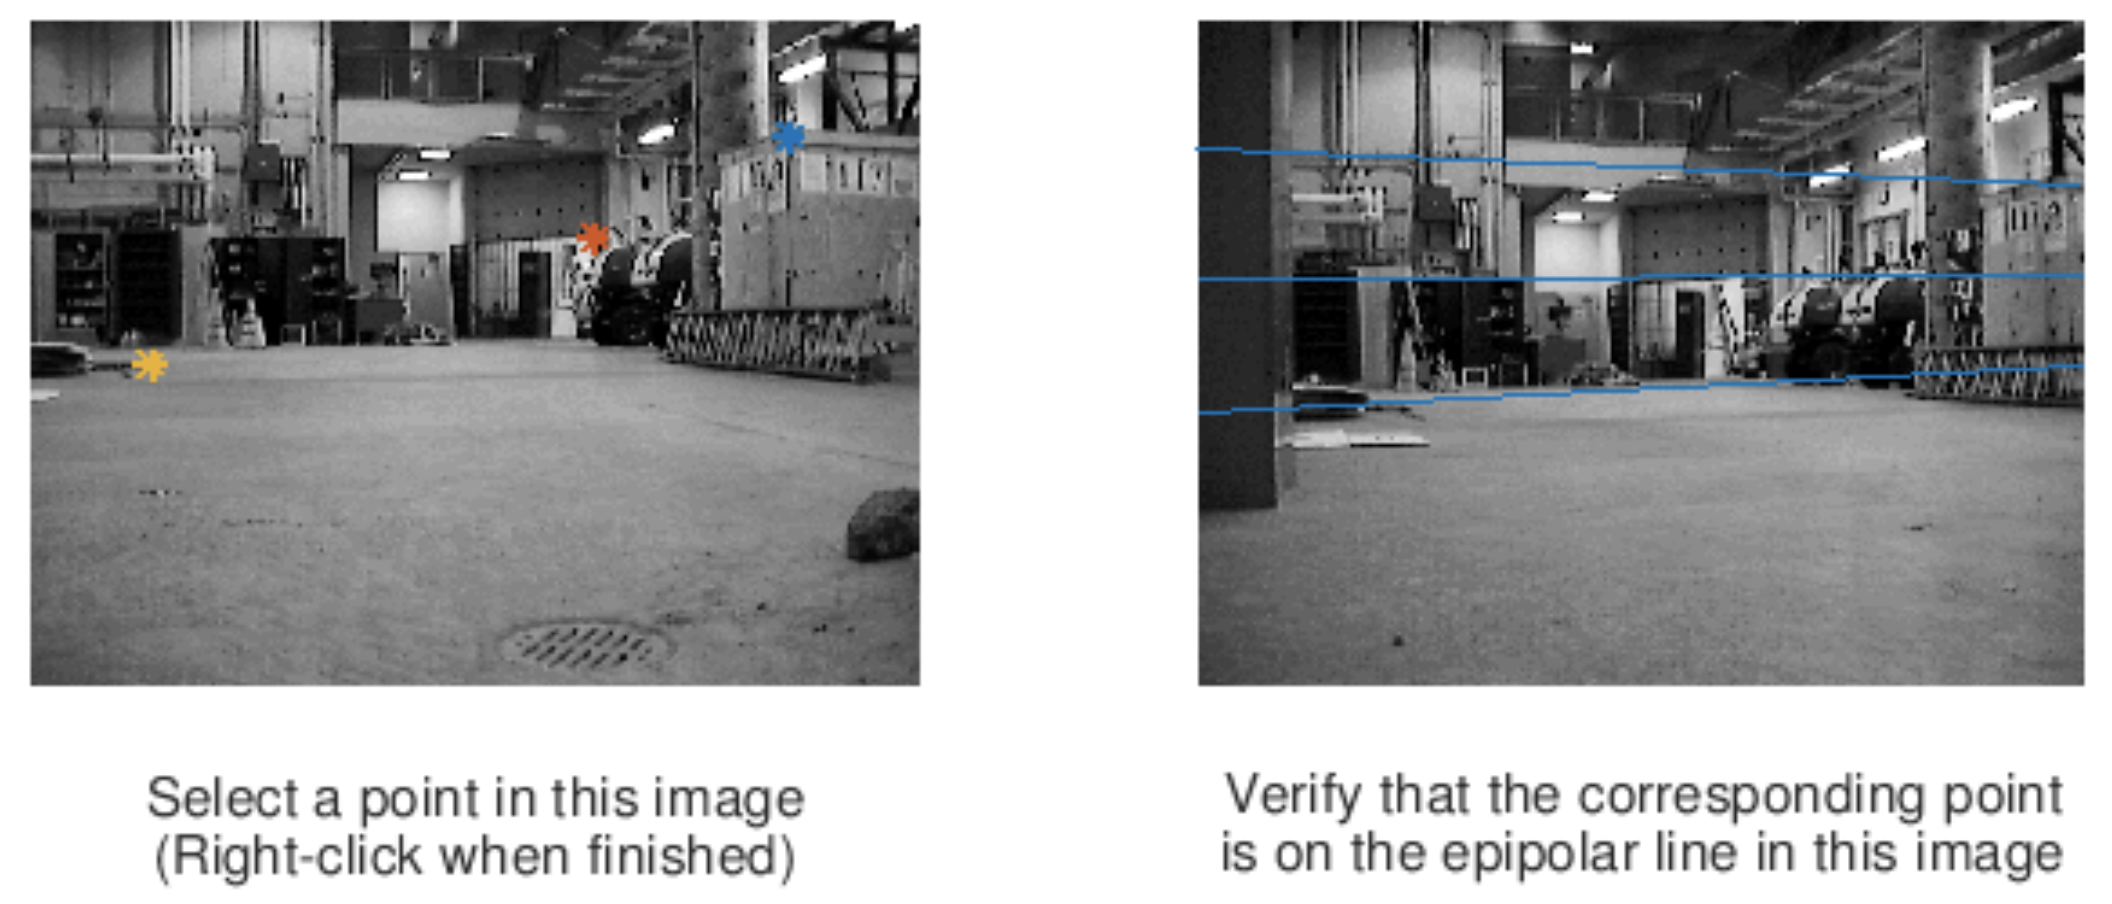
\includegraphics[width=0.85\linewidth]{23_set_result.png}
                \caption{Epipolar lines found by $l_{r} = Fp_{l}$ ($2^{nd}, 3^{rd} $ sets)}
            \end{figure}
        As shown, the results get much better than before in the sense that the corresponding epipolar lines go through the matched points. However, it is a bit strange that the position of the epipole now lies on the right of the second image.\\
        After these experiments, I think that the accuracy of the eight-point algorithm could be quite low if the matching points are not accurately selected. As pointed out in by Hartley \cite{defense}, the inaccuracies in the matching point measurement will result in $A$ not full rank. Consequently, we can only choose the least eigenvector of $A^{T}A$ to be our solution, and this introduce some errors. Although I used Harris feature detector to do the feature matching, there's still inaccuracy in the result. Besides the problem with matching points, this algorithm itself is also not very good. Instead, we can use some iterative algorithm like RANSAC to improve the results.
    \end{solution}
\end{subparts}

\part
\textbf{Final results and structured codes}\\
    To get more accurate results, I used Harris feature detector with more strict requirement and it outputs 17 points for me only. There are supposed to be best matched points and I used these data as input to calculate the fundamental matrix. My final result is shown below:

    \begin{equation}
        F = \left[ \begin{array} { r r r r } { - 3.9335 \mathrm { e } - 09 } & { 6.2600 \mathrm { e } - 07 } & { - 1.1718 \mathrm { e } - 04 } \\ { - 7.6470 \mathrm { e } - 07 } & { - 1.7108 \mathrm { e } - 08 } & { - 1.7488 \mathrm { e } - 03 } \\ { 1.5567 \mathrm { e } - 04 } & { 1.7997 \mathrm { e } - 03 } & { 4.5633 \mathrm { e } - 02 }  \end{array}\right]
    \end{equation}
    The Matlab source codes is attached together with this report, but for your convenience the complete codes for normalization and estimation are listed as follow:
            \begin{lstlisting}
I1 = imread('frc1.tif');
I2 = imread('frc2.tif');
% first computation
displayEpipolarF(I1,I2,estimateF(grp1a', grp1b'))   % transpose since the required input is 2 $\times$ n matrix

% second computation
displayEpipolarF(I1,I2,estimateF([grp2a; grp3a]', [grp2b; grp3b]'))

% final computation using better data omitted...

function [ normalized_pts, T_s ] = normalize( pts )
%   Input: points on an image
%   Output: normalized points for the use of eight_point_algo
    n = size(pts, 1);
    centroid = sum(pts, 1) / n;
    disp('The centroid is');
    disp(centroid);
    
    pts_demean = pts - centroid;
    
    squared_distance_sum = sum(sum(pts_demean.^2));
    
    scale_factor = sqrt(mean(squared_distance_sum) / 2);    % scale to sqrt(2)
    
    normalized_pts = pts_demean / scale_factor;
    
    disp('Check for the RMS average distance:');
    disp(sqrt(mean(sum(sum(normalized_pts.^2)))));
    
    % x' = s * (x + t_x) ; y' = s * (y + t_y)
    t_x = -centroid(1);
    t_y = -centroid(2);
    s = 1 / scale_factor;
    
    T_s = [s 0 s*t_x; 0 s s*t_y; 0 0 1];
    disp('The similarity transformation is');
    disp(T_s);
end


function F = estimateF(x1, x2)
    % x1 and x2 are each 2 x n matrices with the 
    % columns corresponding to the coordinates in the first
    % and the second image respectively
    pts1 = x1';
    pts2 = x2';
    
    [n_pts1, T_s1] = normalize(pts1);
    [n_pts2, T_s2] = normalize(pts2);
    
    % construct A
    A = [n_pts2(:,1).*n_pts1(:,1) n_pts2(:,1).*n_pts1(:,2) n_pts2(:,1) n_pts2(:,2).*n_pts1(:,1) n_pts2(:,2).*n_pts1(:,2) n_pts2(:,2) n_pts1(:,1) n_pts1(:,2) ones(size(n_pts1(:,1)))];
    % from svd(A), get F
    [U, S, V] = svd(A);
    F_temp = V(:,length(V));
    F_temp = reshape(F_temp, [3,3])';
    % enforce F singularity
    [U_f, S_f, V_f] = svd(F_temp);
    S_f(3,3) = 0;
    F_prime = U_f * S_f * V_f';
    
    %denormalization
    F = T_s2' * F_prime * T_s1;
end
        \end{lstlisting}
    
    \begin{figure}[H]
    \centering
    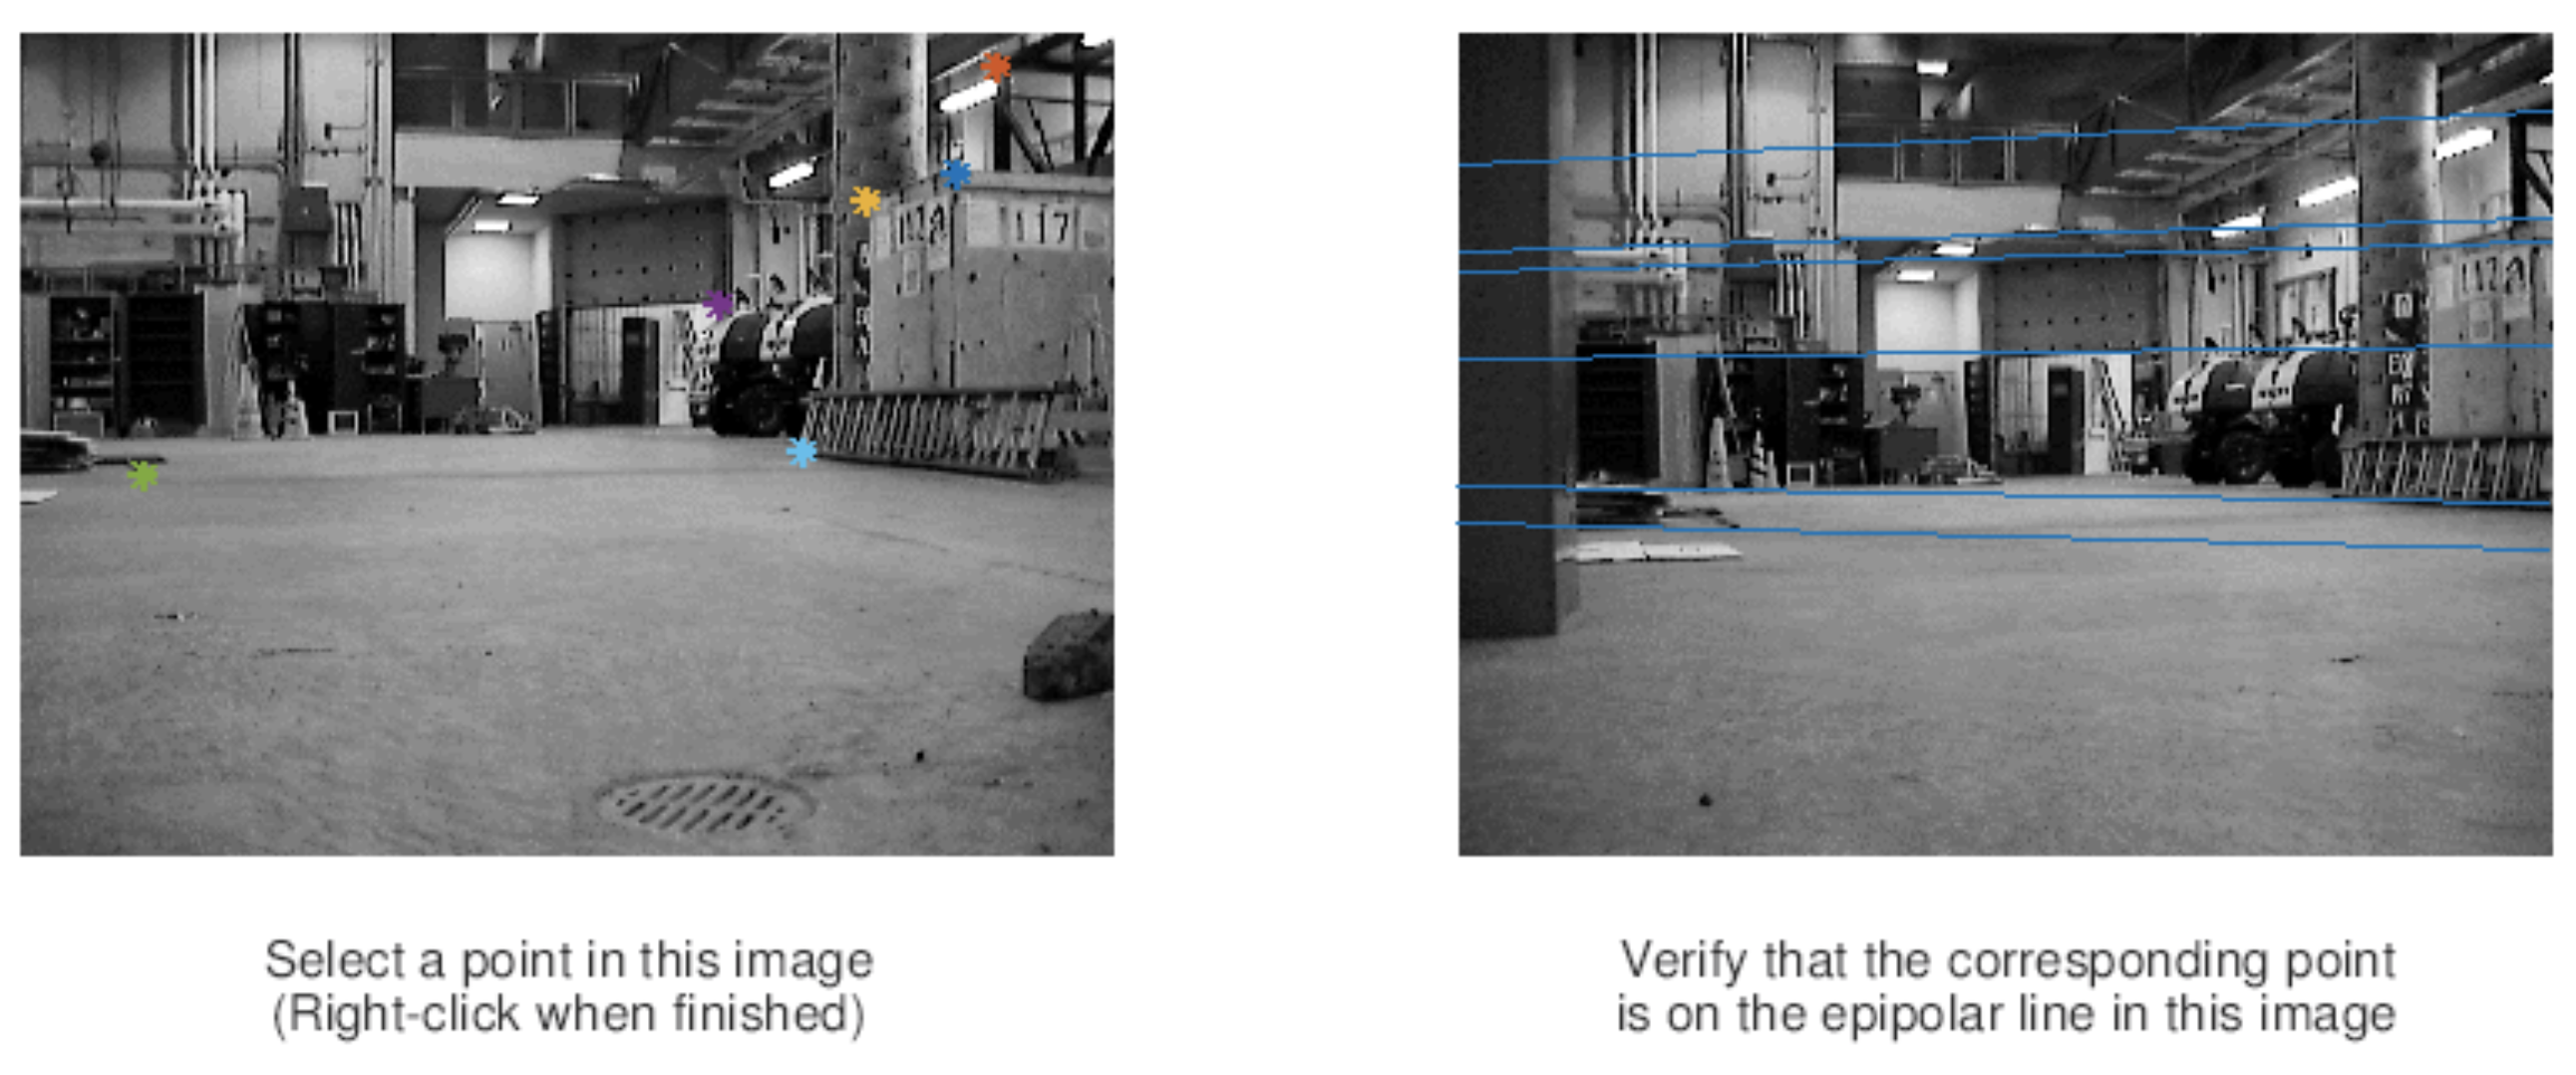
\includegraphics[width=0.85\linewidth]{visualize.png}
    \caption{Final (best) result}
    \end{figure}
    The figure above shows that for every point selected in the left image, the fundamental matrix can effectively find the corresponding epipolar line in the right image. This is obtained use the most accurate matched points I can get.
\end{parts}
\end{questions}